\chapter{Operational parameter exploration and their implications}

\section{Introduction}

Building on the foundations laid by the preceding chapters, this chapter delves into a more nuanced investigation of the parametric influences on the resulting force curves obtained through Atomic Force Microscopy (AFM). When operating an AFM, it is typical to use a standard set of operational parameters. \cite{Schirmeisen2007} These parameters are often found during operation in an exploratory manner to find a good signal to noise ratio. However, it can be prudent  to examine a spectrum of force curves under varied conditions. Such an investigation enables the assessment of result consistency across diverse settings, thereby ensuring that the observed outcomes are not merely artifacts of parameter-specific minima phenomena. Additionally, a range of differing conditions can provide an insight into how other phenomena may have an effect on the observed behaviour of the curves.

A range of differing conditions were repeated with the following parameter changes: Tip speed, dwell time, solution pH and forcemapping. 

\subsubsection{Tip Speed Variations}
The velocity of the AFM tip's approach and retraction impacts the force measurements, potentially altering the energy landscape of particle interactions. Varying the tip speed not only affects the kinetic parameters but also provides insight into time-dependent phenomena such as lubrication forces and simple viscous drag. The adjustment of the tip's velocity probes the dynamic response of the system, shedding light on the viscoelastic properties of the medium and the rate-dependent behavior of interparticle forces.

\subsubsection{Effect of Dwell Time}

The incorporation of a 5-second dwell time between the approach and retrace allows for the relaxation of the system and the establishment of equilibrium conditions in between movements, potentially revealing the subtleties of time-dependent interactions. The extended dwell time is expected to amplify phenomena such as capillary forces and hydration layers, which are often overshadowed by more dominant forces in quicker measurements.

\subsubsection{Solution pH Influence}

The pH of the colloidal solution is a determinant of the surface charge on the silica particles, which in turn modulates the force interactions observed. The variations in pH are expected to impact the electrical double layer, thereby influencing the force profiles and interaction potentials, while retaining the same force curve profile ranges as shown previously.

\subsubsection{Forcemapping for wide range site analysis}

Forcemapping, a method of tracking force-distance curves over a defined grid area, was employed to obtain a comprehensive understanding of the force distribution across the sample. This technique is useful in discerning how heterogenious the analysed surface is and provides a statistical interpretation of interparticle forces across a range of areas.

The exploration of these parameters serves not just as a methodical inquiry into the forces acting within colloidal dispersions, but also as a means to justify our approach to force curve analysis. The diversity of these conditions reflects the complex nature of the studied system and underscores the need for a comprehensive dataset that accurately represents the multifaceted nature of particle interactions.

The subsequent section presents the force distributions across our dataset, providing empirical evidence to the impact of these discussed factors. Finally, the section highlights the differences between the "standard" dataset and the modified parameters.

\section{Tip speed analysis}

One of the differences between the different tip speeds was the data density. For faster speed less data was taken, while slower speeds had more data taken. This was due to the rate in which the AFM takes in data - the AFM was set to take in the maximum rate of data throughout the whole process. This was done to maximise the volume of data usable for the binning process (as seen in chapter 5). 

For 0.1 and 0.5Hz, the data rate was more than enough the support the processing of the curves, while 2Hz had significantly less data, and required a more involved fitting, with generally a lower bitsize setting used in the script - increasing the noise in the averaged curve.


% 0.6mM Section
\subsubsection*{0.6mM}
For 0.6mM only one site was used. I don't have
\begin{figure}[h!]
\centering
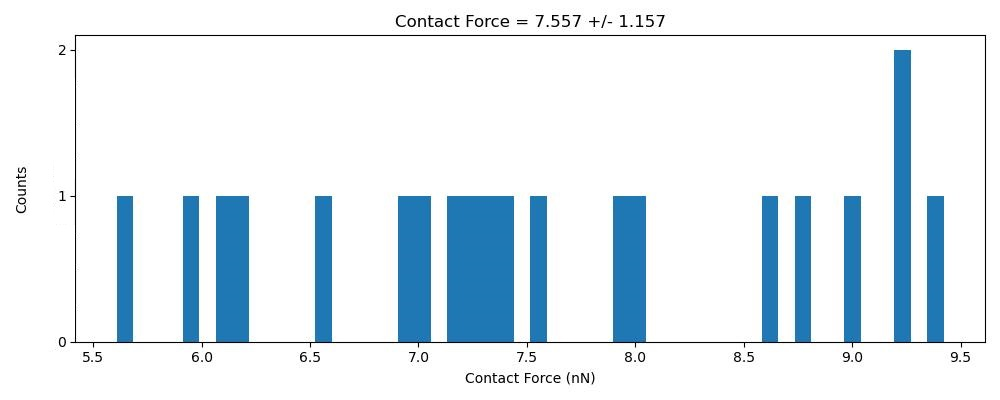
\includegraphics[width=\textwidth]{chapter7/Tip speed/0.6mM/approach_f_c_hist.jpg}
\caption{Approach force-current histogram at 0.6mM}
\end{figure}

\begin{figure}[h!]
\centering
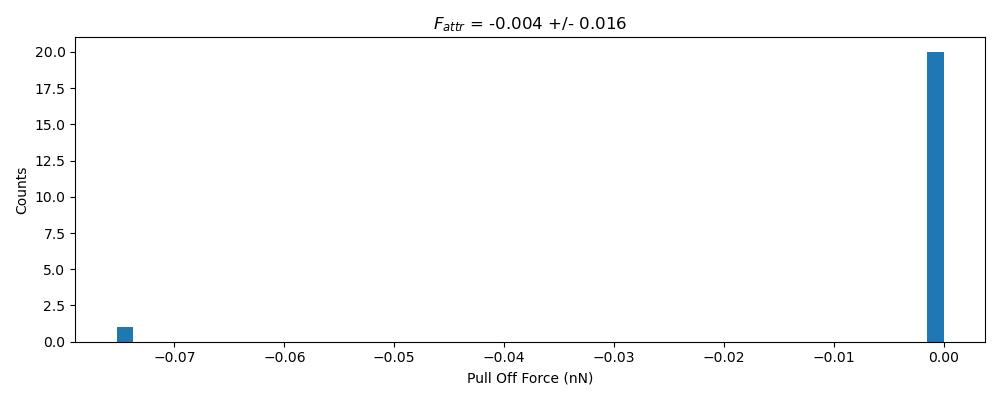
\includegraphics[width=\textwidth]{chapter7/Tip speed/0.6mM/retract_f_a_hist.jpg}
\caption{Retract force-amplitude histogram at 0.6mM}
\end{figure}
text
\newpage

% 1.6mM Section
\subsubsection*{1.6mM}
\begin{figure}[h!]
\centering
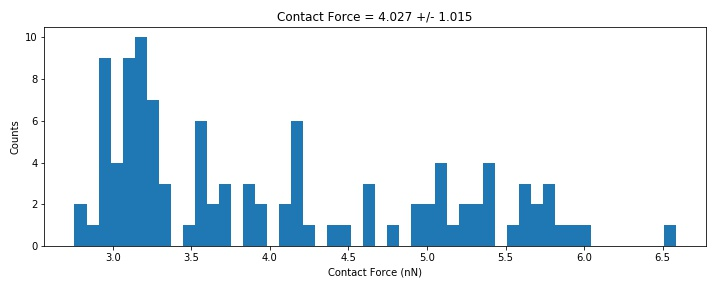
\includegraphics[width=\textwidth]{chapter7/Tip speed/1.6mM/S1 2Hz/approach_f_c_hist.jpg}
\caption{Approach curve for 1.6mM, S2 at 2Hz}
\end{figure}

\begin{figure}[h!]
\centering
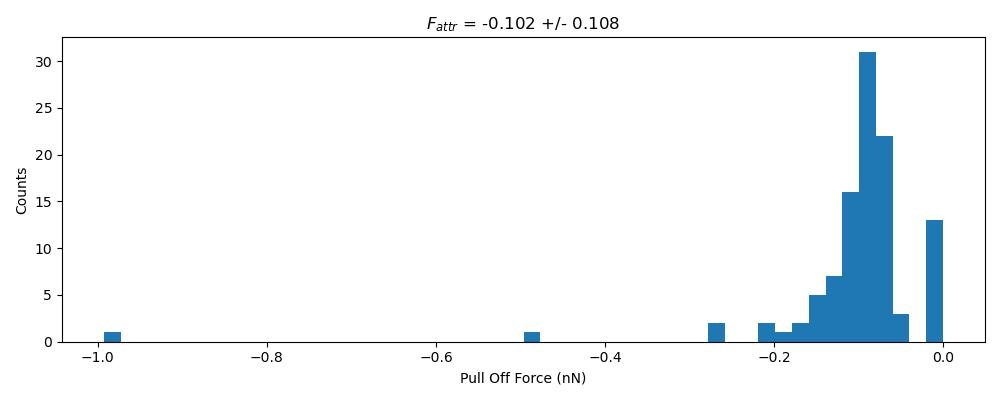
\includegraphics[width=\textwidth]{chapter7/Tip speed/1.6mM/S1 2Hz/retract_f_a_hist.jpg}
\caption{Retract curve for 1.6mM, S2 at 2Hz}
\end{figure}
text
\newpage

% 5mM Section
\subsubsection*{5mM}
\paragraph{S1 2Hz}
\begin{figure}[h!]
\centering
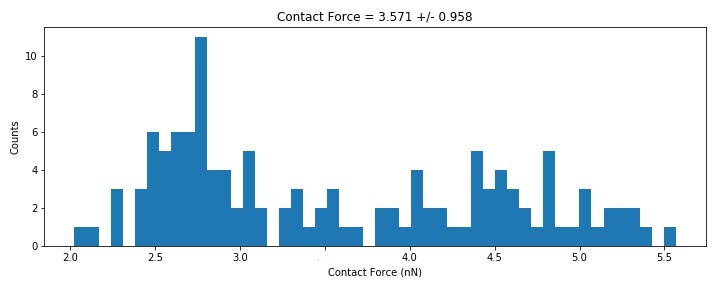
\includegraphics[width=\textwidth]{chapter7/Tip speed/5mM/S1 2Hz/approach_f_c_hist.jpg}
\caption{Approach curve for 5mM, S1 at 2Hz}
\end{figure}

\begin{figure}[h!]
\centering
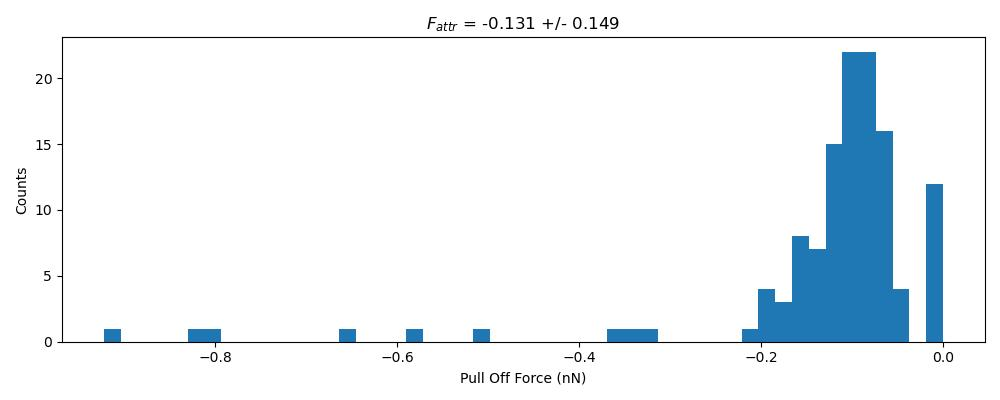
\includegraphics[width=\textwidth]{chapter7/Tip speed/5mM/S1 2Hz/retract_f_a_hist.jpg}
\caption{Retract curve for 5mM, S1 at 2Hz}
\end{figure}
text
\newpage

\paragraph{S2 2Hz}
\begin{figure}[h!]
\centering
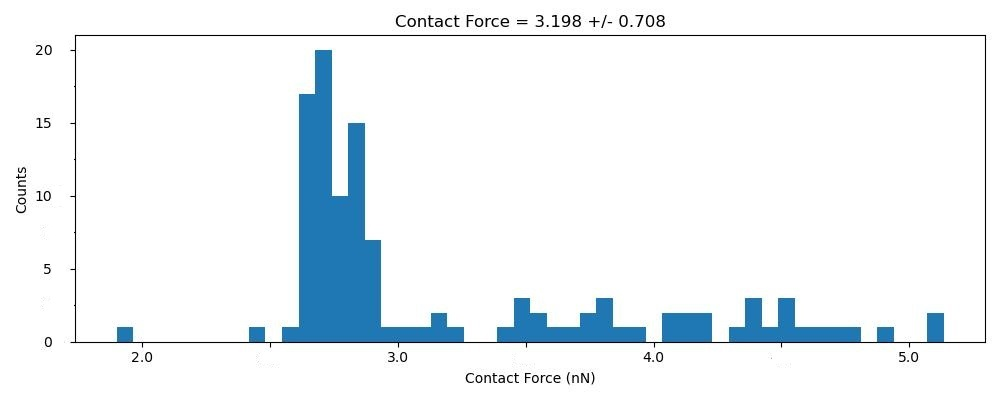
\includegraphics[width=\textwidth]{chapter7/Tip speed/5mM/S2 2Hz/approach_f_c_hist.jpg}
\caption{Approach curve for 5mM, S2 at 2Hz}
\end{figure}

\begin{figure}[h!]
\centering
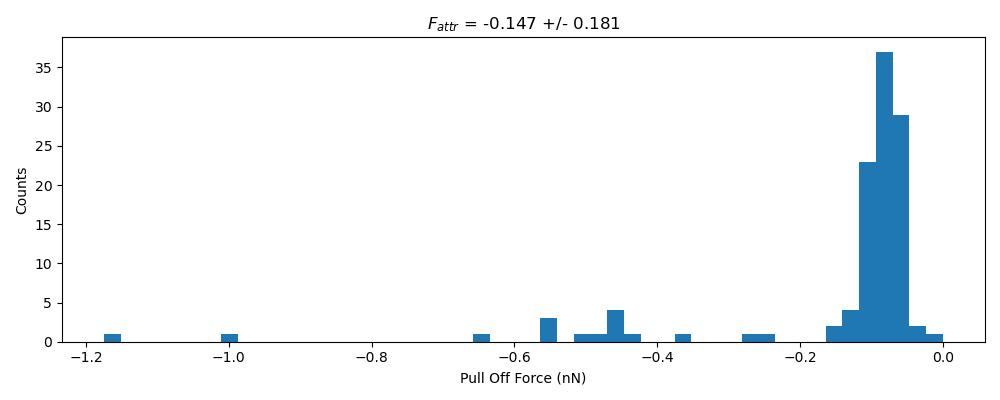
\includegraphics[width=\textwidth]{chapter7/Tip speed/5mM/S2 2Hz/retract_f_a_hist.jpg}
\caption{Retract curve for 5mM, S2 at 2Hz}
\end{figure}
text
\newpage

\paragraph{S3 2Hz}
\begin{figure}[h!]
\centering
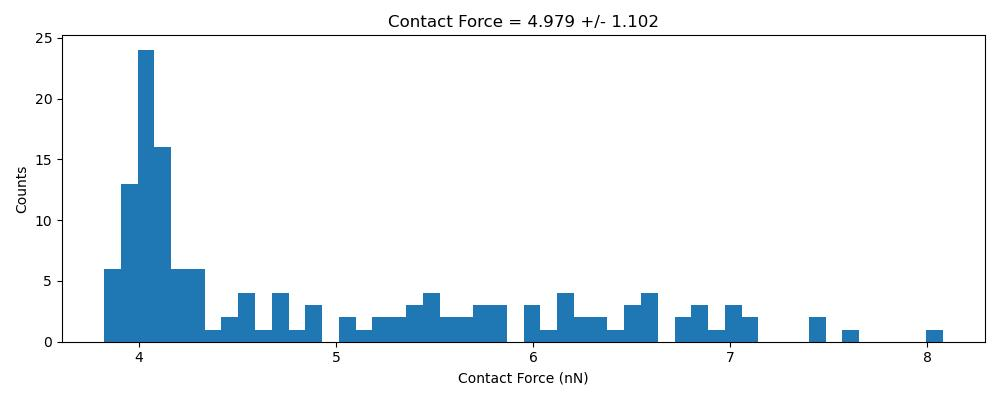
\includegraphics[width=\textwidth]{chapter7/Tip speed/5mM/S3 2Hz/approach_f_c_hist.jpg}
\caption{Approach curve for 5mM, S3 at 2Hz}
\end{figure}

\begin{figure}[h!]
\centering
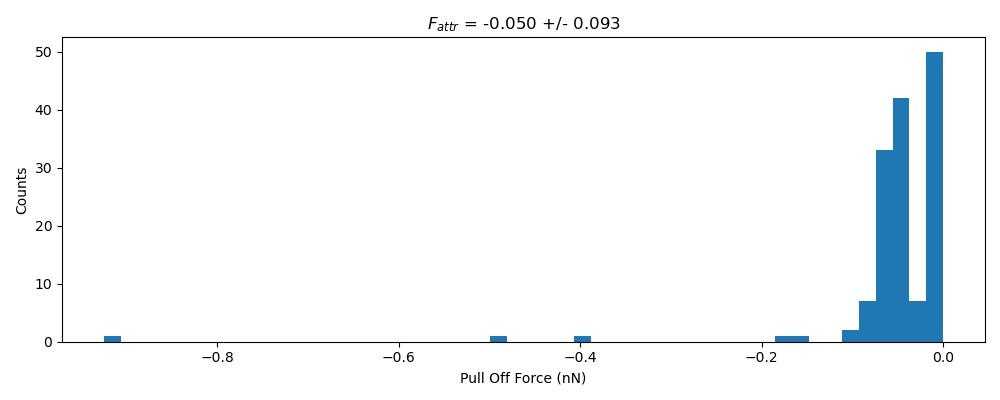
\includegraphics[width=\textwidth]{chapter7/Tip speed/5mM/S3 2Hz/retract_f_a_hist.jpg}
\caption{Retract curve for 5mM, S3 at 2Hz}
\end{figure}
text
\newpage

% 10mM Section
\subsubsection*{10mM}
\paragraph{S1 0.1Hz}
\begin{figure}[h!]
\centering
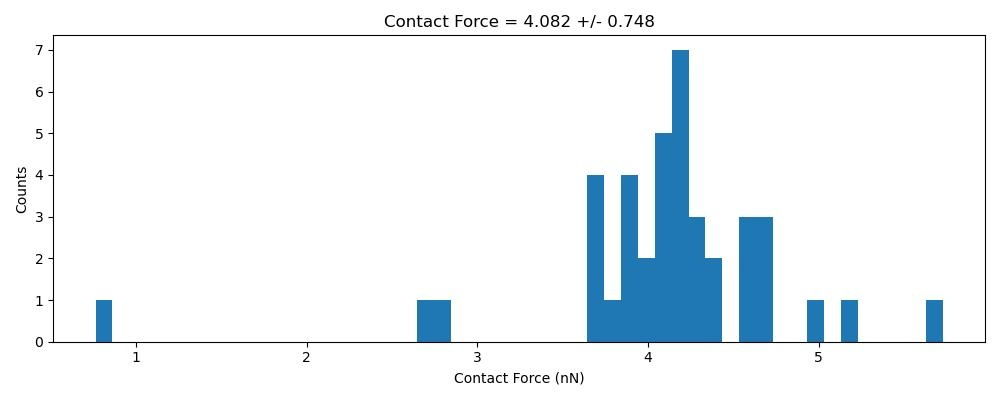
\includegraphics[width=\textwidth]{chapter7/Tip speed/10mM/S1 0.1Hz/approach_f_c_hist.jpg}
\caption{Approach curve for 10mM, S1 at 0.1Hz}
\end{figure}

\begin{figure}[h!]
\centering
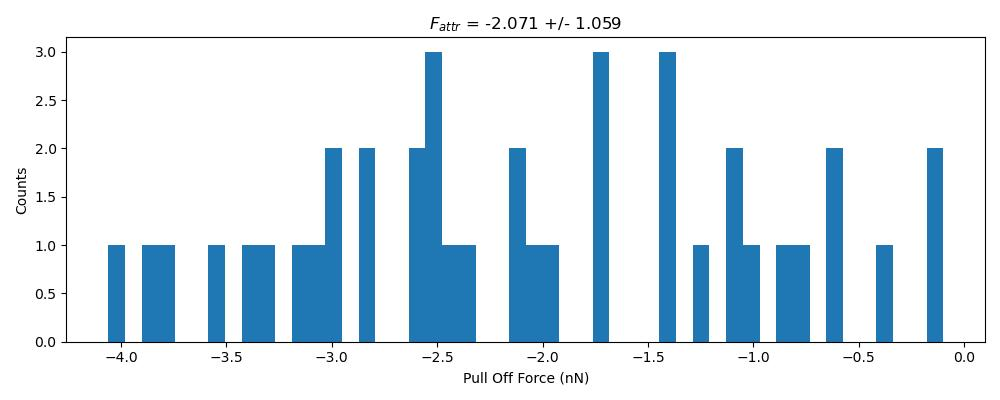
\includegraphics[width=\textwidth]{chapter7/Tip speed/10mM/S1 0.1Hz/retract_f_a_hist.jpg}
\caption{Retract curve for 10mM, S1 at 0.1Hz}
\end{figure}
text
\newpage

\paragraph{S1 2Hz}
\begin{figure}[h!]
\centering
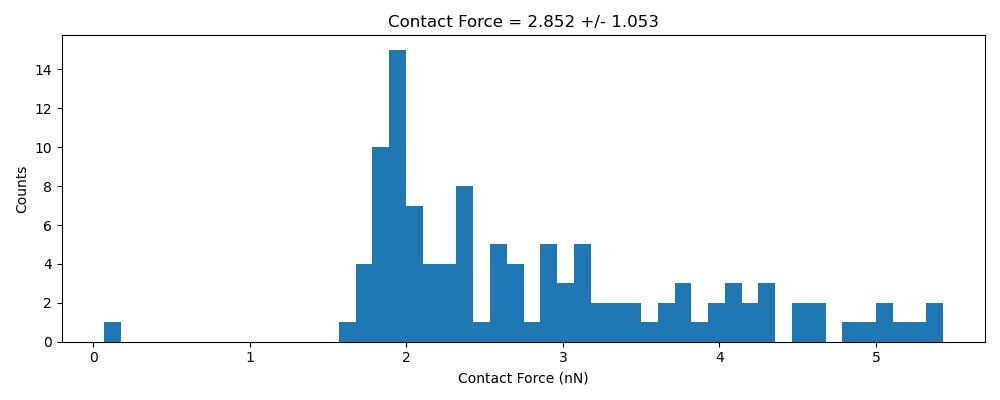
\includegraphics[width=\textwidth]{chapter7/Tip speed/10mM/S1 2Hz/approach_f_c_hist.jpg}
\caption{Approach curve for 10mM, S1 at 2Hz}
\end{figure}

\begin{figure}[h!]
\centering
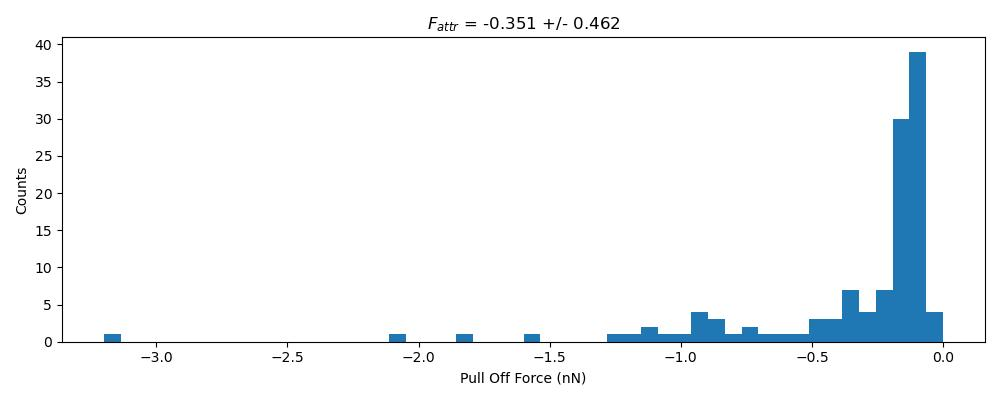
\includegraphics[width=\textwidth]{chapter7/Tip speed/10mM/S1 2Hz/retract_f_a_hist.jpg}
\caption{Retract curve for 10mM, S1 at 2Hz}
\end{figure}
text
\newpage

\paragraph{S2 0.1Hz}
\begin{figure}[h!]
\centering
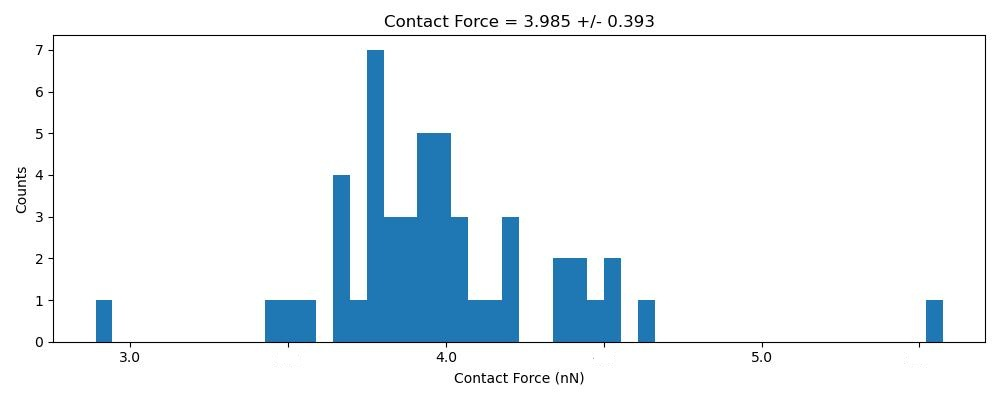
\includegraphics[width=\textwidth]{chapter7/Tip speed/10mM/S2 0.1Hz/approach_f_c_hist.jpg}
\caption{Approach curve for 10mM, S2 at 0.1Hz}
\end{figure}

\begin{figure}[h!]
\centering
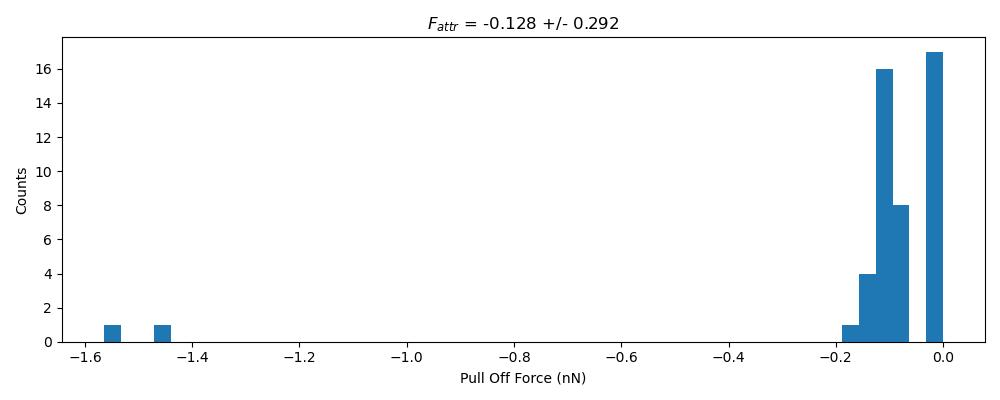
\includegraphics[width=\textwidth]{chapter7/Tip speed/10mM/S2 0.1Hz/retract_f_a_hist.jpg}
\caption{Retract curve for 10mM, S2 at 0.1Hz}
\end{figure}
text
\newpage

\begin{figure}[h!]
\centering
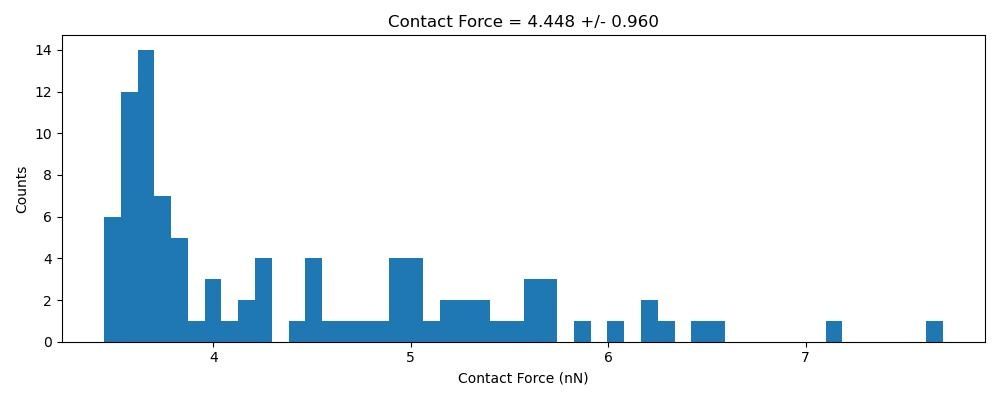
\includegraphics[width=\textwidth]{chapter7/Tip speed/10mM/S2 2Hz/approach_f_c_hist.jpg}
\caption{Approach curve for 10mM, S2 at 2Hz}
\end{figure}

\begin{figure}[h!]
\centering
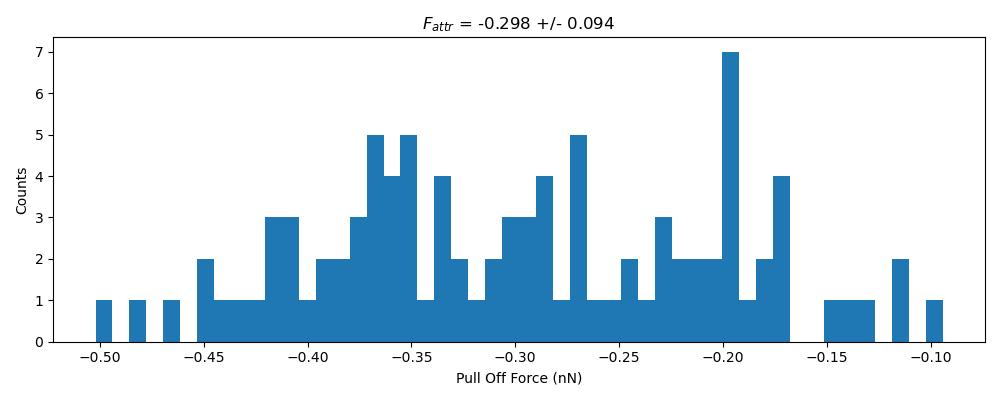
\includegraphics[width=\textwidth]{chapter7/Tip speed/10mM/S2 2Hz/retract_f_a_hist.jpg}
\caption{Retract curve for 10mM, S2 at 2Hz}
\end{figure}
text
\newpage

\paragraph{S3 0.1Hz}
\begin{figure}[h!]
\centering
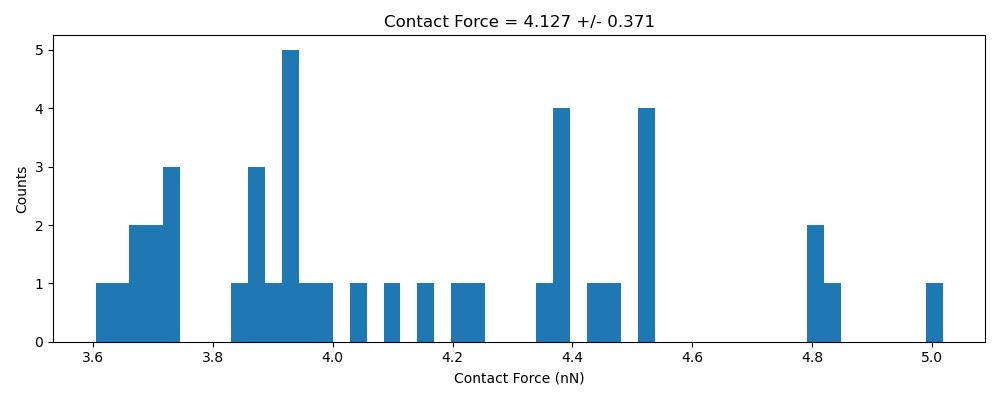
\includegraphics[width=\textwidth]{chapter7/Tip speed/10mM/S3 0.1Hz/approach_f_c_hist.jpg}
\caption{Approach curve for 10mM, S3 at 0.1Hz}
\end{figure}

\begin{figure}[h!]
\centering
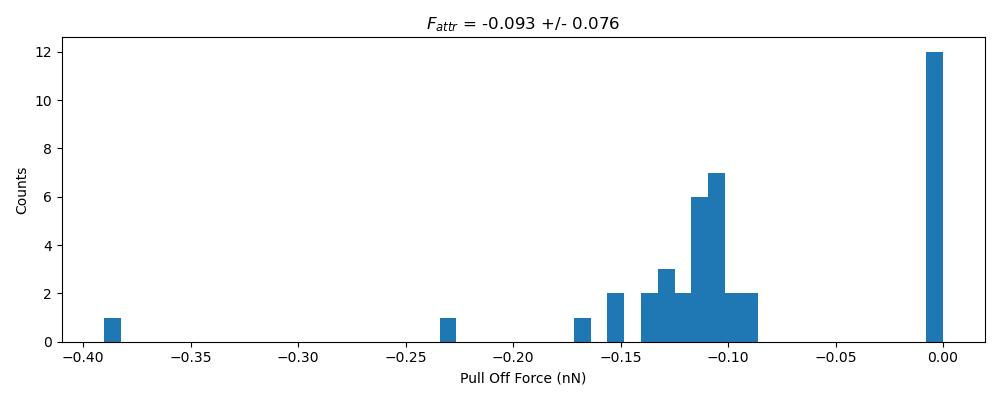
\includegraphics[width=\textwidth]{chapter7/Tip speed/10mM/S3 0.1Hz/retract_f_a_hist.jpg}
\caption{Retract curve for 10mM, S3 at 0.1Hz}
\end{figure}
text
\newpage

\paragraph{S3 2Hz}
\begin{figure}[h!]
\centering
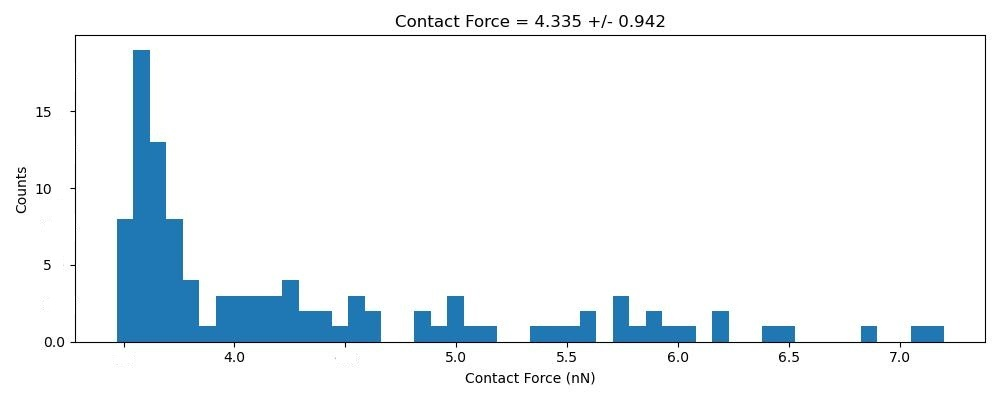
\includegraphics[width=\textwidth]{chapter7/Tip speed/10mM/S3 2Hz/approach_f_c_hist.jpg}
\caption{Approach curve for 10mM, S3 at 2Hz}
\end{figure}

\begin{figure}[h!]
\centering
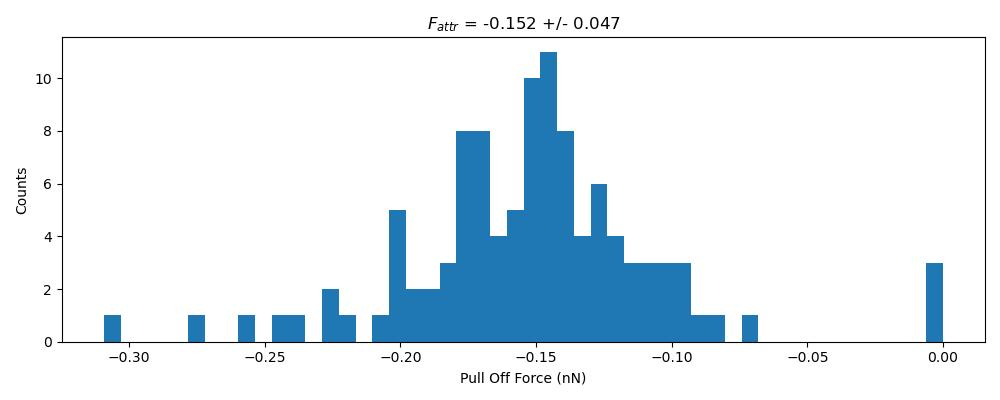
\includegraphics[width=\textwidth]{chapter7/Tip speed/10mM/S3 2Hz/retract_f_a_hist.jpg}
\caption{Retract curve for 10mM, S3 at 2Hz}
\end{figure}
text
\newpage

% 25mM Section
\subsubsection*{25mM}
\paragraph{S1 2Hz}
\begin{figure}[h!]
\centering
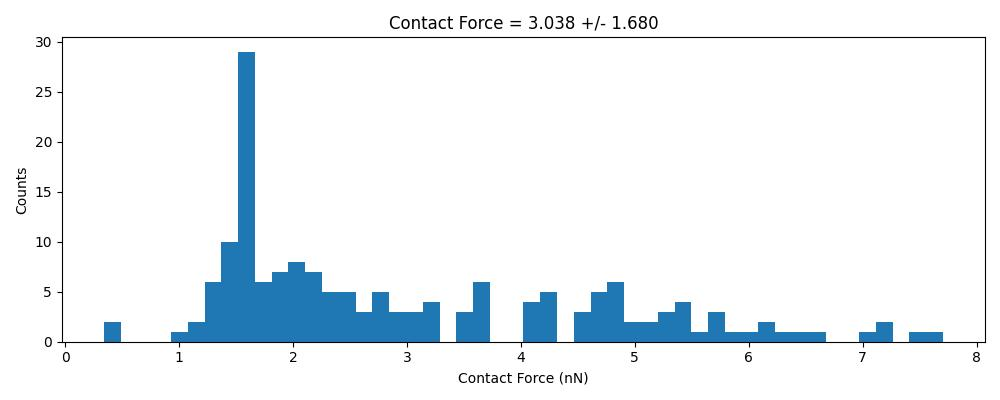
\includegraphics[width=\textwidth]{chapter7/Tip speed/25mM/S1 2Hz/approach_f_c_hist.jpg}
\caption{Approach curve for 25mM, S1 at 2Hz}
\end{figure}

\begin{figure}[h!]
\centering
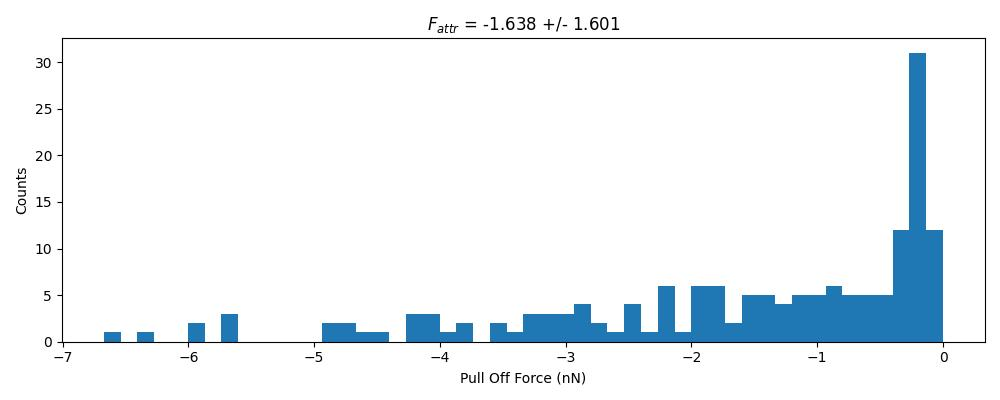
\includegraphics[width=\textwidth]{chapter7/Tip speed/25mM/S1 2Hz/retract_f_a_hist.jpg}
\caption{Retract curve for 25mM, S1 at 2Hz}
\end{figure}
text
\newpage

\paragraph{S2 2Hz}
\begin{figure}[h!]
\centering
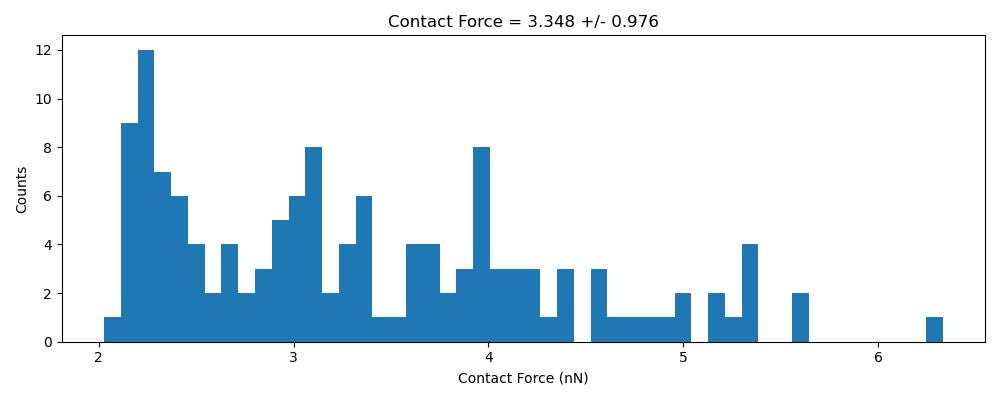
\includegraphics[width=\textwidth]{chapter7/Tip speed/25mM/S2 2Hz/approach_f_c_hist.jpg}
\caption{Approach curve for 25mM, S2 at 2Hz}
\end{figure}

\begin{figure}[h!]
\centering
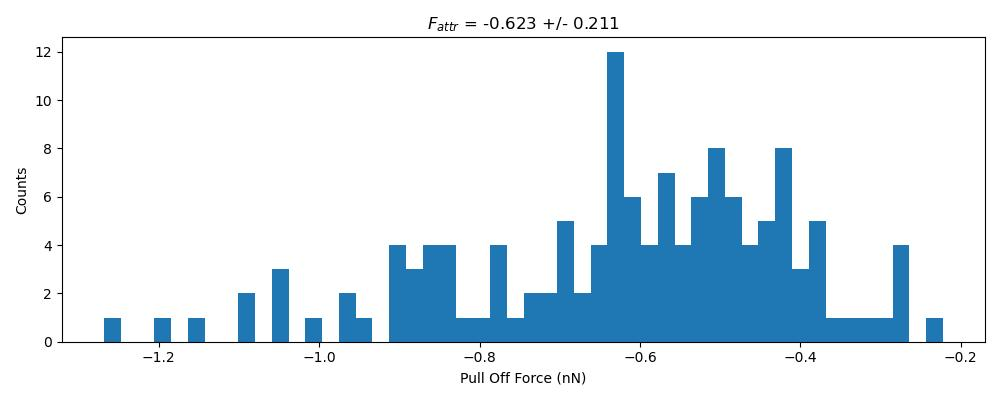
\includegraphics[width=\textwidth]{chapter7/Tip speed/25mM/S2 2Hz/retract_f_a_hist.jpg}
\caption{Retract curve for 25mM, S2 at 2Hz}
\end{figure}
text
\newpage

\paragraph{S3 2Hz}
\begin{figure}[h!]
\centering
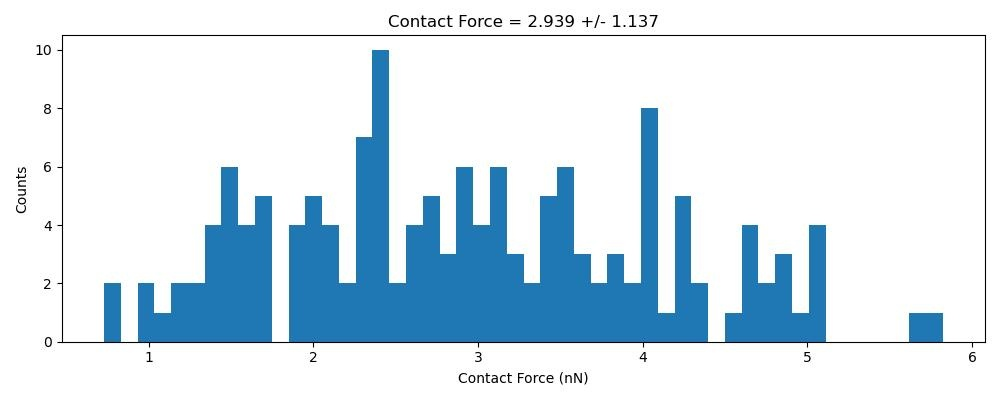
\includegraphics[width=\textwidth]{chapter7/Tip speed/25mM/S3 2Hz/approach_f_c_hist.jpg}
\caption{Approach curve for 25mM, S3 at 2Hz}
\end{figure}

\begin{figure}[h!]
\centering
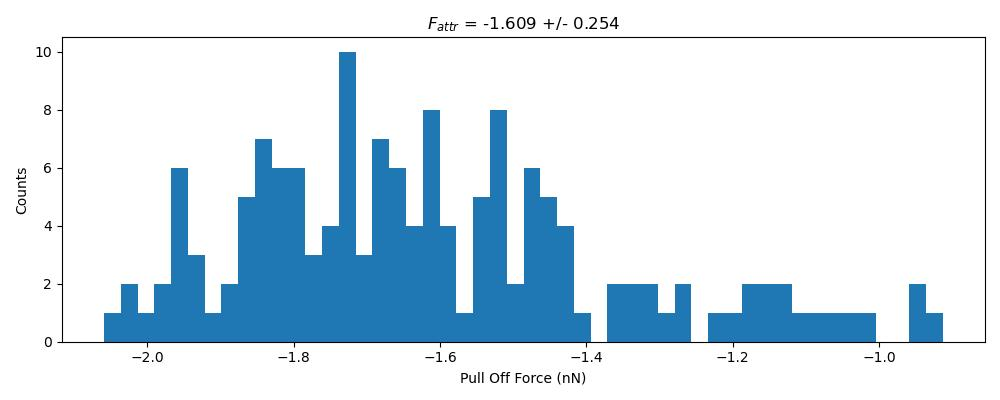
\includegraphics[width=\textwidth]{chapter7/Tip speed/25mM/S3 2Hz/retract_f_a_hist.jpg}
\caption{Retract curve for 25mM, S3 at 2Hz}
\end{figure}
text
\newpage

% 230mM Section
\subsubsection*{230mM}
\paragraph{S1 2Hz}
\begin{figure}[h!]
\centering
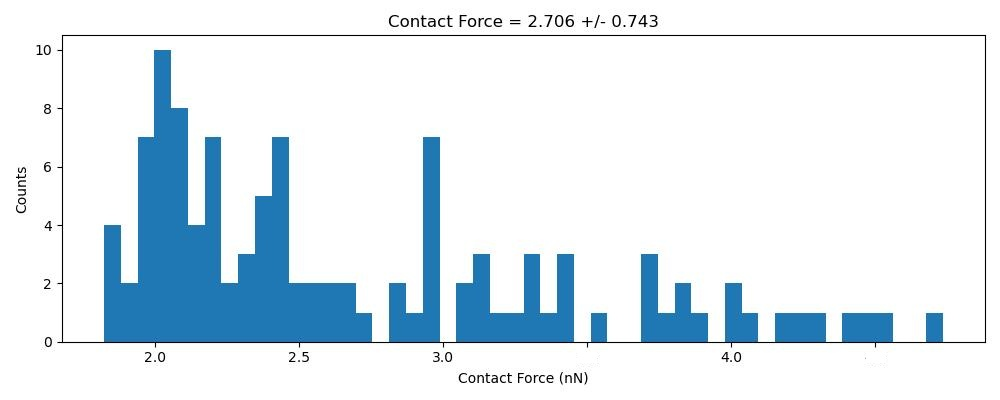
\includegraphics[width=\textwidth]{chapter7/Tip speed/230mM/S1 2Hz/approach_f_c_hist.jpg}
\caption{Approach curve for 230mM, S1 at 2Hz}
\end{figure}

\begin{figure}[h!]
\centering
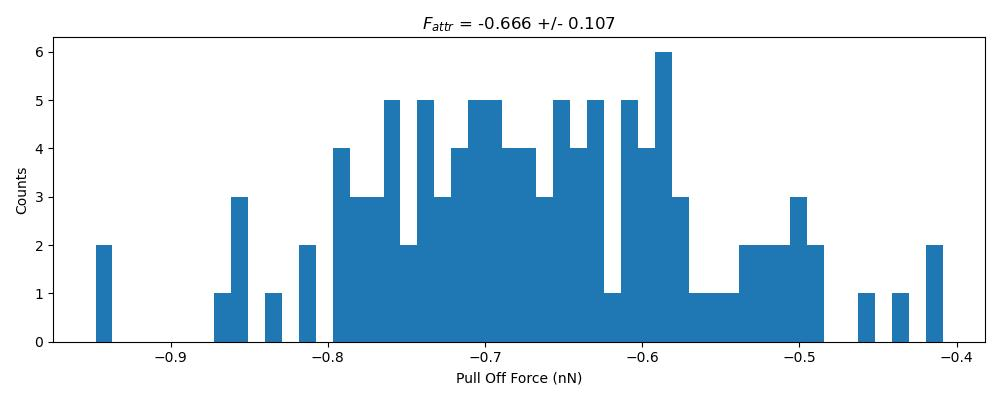
\includegraphics[width=\textwidth]{chapter7/Tip speed/230mM/S1 2Hz/retract_f_a_hist.jpg}
\caption{Retract curve for 230mM, S1 at 2Hz}
\end{figure}
text
\newpage

\paragraph{S2 2Hz}
\begin{figure}[h!]
\centering
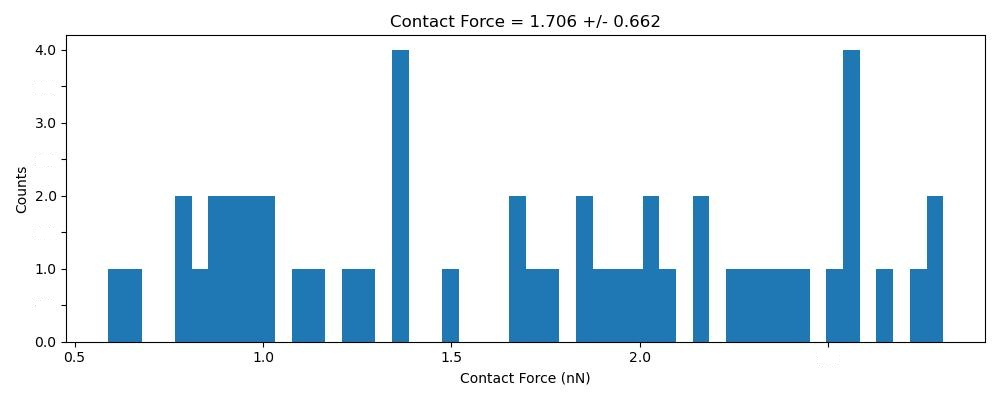
\includegraphics[width=\textwidth]{chapter7/Tip speed/230mM/S2 2Hz/approach_f_c_hist.jpg}
\caption{Approach curve for 230mM, S2 at 2Hz}
\end{figure}

\begin{figure}[h!]
\centering
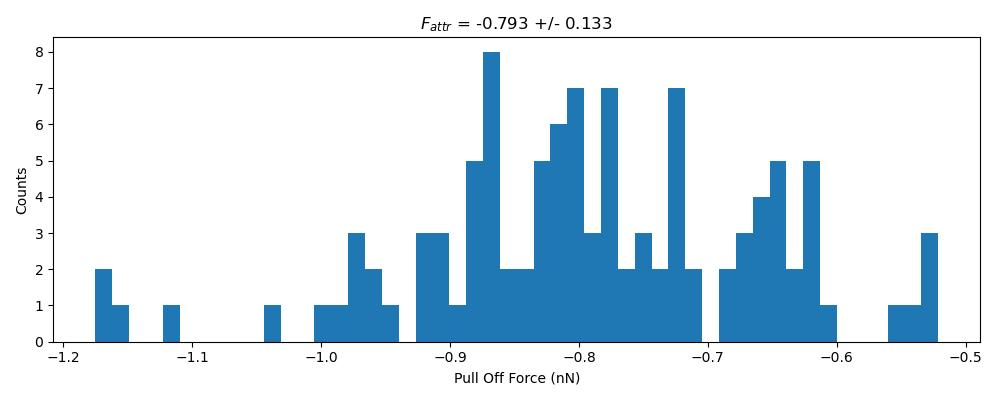
\includegraphics[width=\textwidth]{chapter7/Tip speed/230mM/S2 2Hz/retract_f_a_hist.jpg}
\caption{Retract curve for 230mM, S2 at 2Hz}
\end{figure}
text
\newpage

% 550mM Section
\subsubsection*{550mM}
\paragraph{S2 2Hz}
\begin{figure}[h!]
\centering
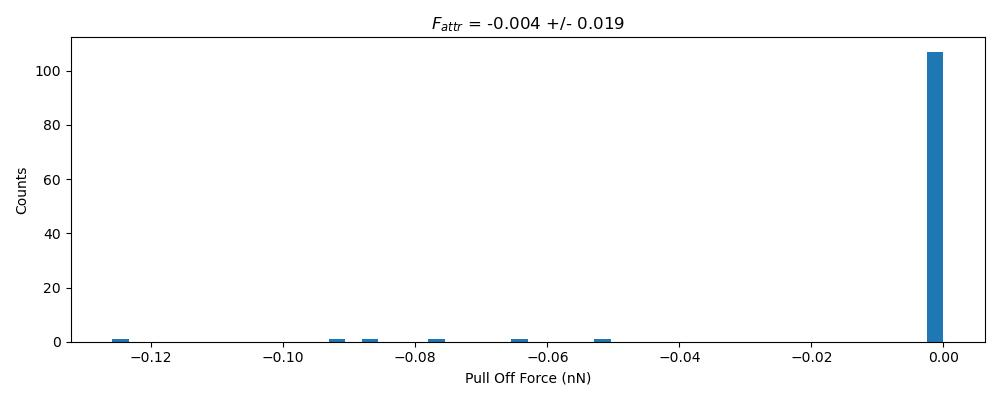
\includegraphics[width=\textwidth]{chapter7/Tip speed/550mM/S2 2Hz/approach_f_a_hist.jpg}
\caption{Approach curve for 550mM, S2 at 2Hz}
\end{figure}

\begin{figure}[h!]
\centering
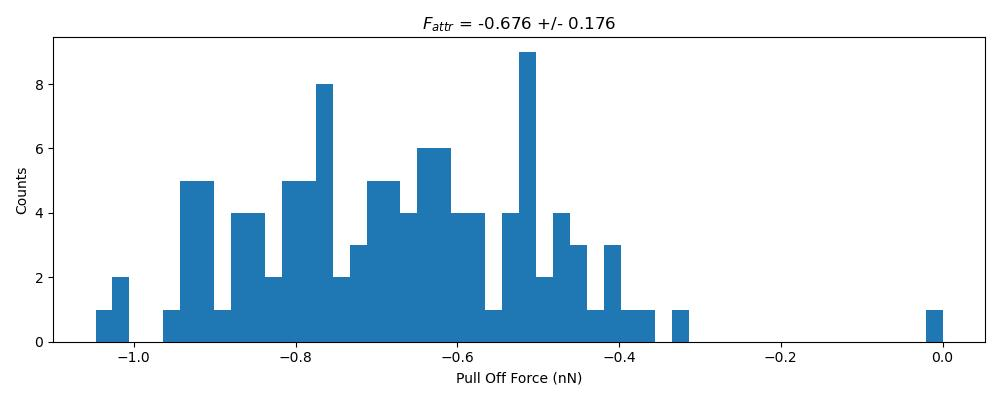
\includegraphics[width=\textwidth]{chapter7/Tip speed/550mM/S2 2Hz/retract_f_a_hist.jpg}
\caption{Retract curve for 550mM, S2 at 2Hz}
\end{figure}

\paragraph{S3 2Hz}
\begin{figure}[h!]
\centering
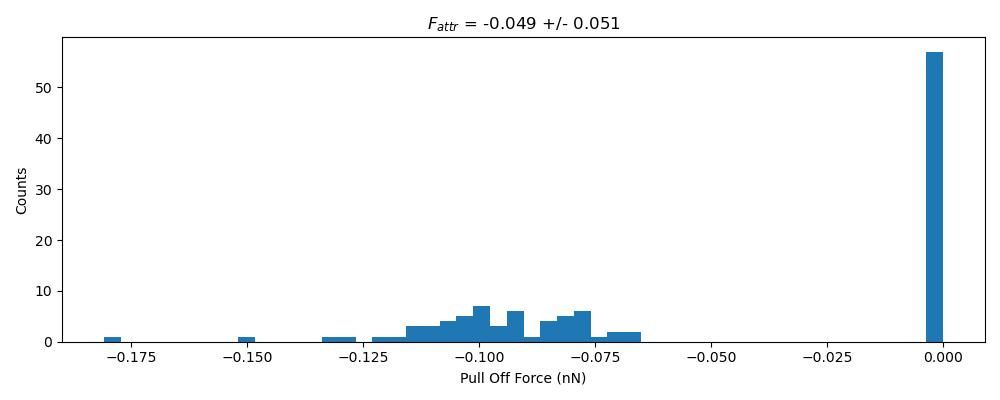
\includegraphics[width=\textwidth]{chapter7/Tip speed/550mM/S3 2Hz/approach_f_a_hist.jpg}
\caption{Approach curve for 550mM, S3 at 2Hz}
\end{figure}

\begin{figure}[h!]
\centering
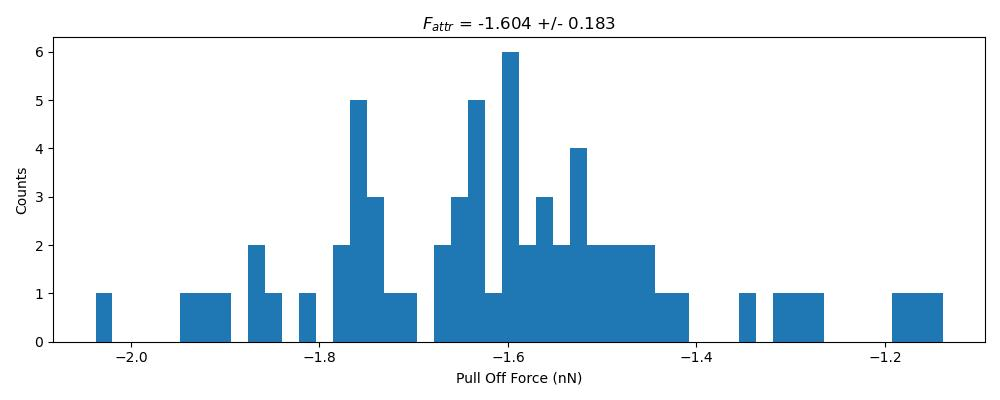
\includegraphics[width=\textwidth]{chapter7/Tip speed/550mM/S3 2Hz/retract_f_a_hist.jpg}
\caption{Retract curve for 550mM, S3 at 2Hz}
\end{figure}




\section{JPK Forcemapping}

One of the limitations of using the interpertaion software is that it assumes that all curves are of the same shape. This is not the case for a range of sites.

Due to the differences between the AFMs, and potentially the way the AFMs were used to measure the interactions, the "shelf" seen was more of a snap to contact point in the curve. This meant that the shelf seen in the previous AFM, may have been the point in which the tip snapped to the surface, and the older AFM may not have been able to detect or measure this sudden change in the way the new one has. 

Due to the limited window in which this AFM was available, it was not possible to explore this interaction further, but it is promising that this shelf feature is present across multiple AFMs and sites.

Todo:

- Write force map analysis
- Write shelf analysis tool
